\documentclass[UTF8,a4paper,zihao=-4]{ctexart}

\usepackage[margin=2cm]{geometry}
\usepackage{amsmath,amssymb}
\usepackage{graphicx}
\usepackage{caption}
\usepackage{subcaption}
\usepackage{booktabs}
\usepackage{array}
\usepackage{float}
\usepackage{hyperref}
\usepackage{xcolor}

\graphicspath{{figures/}}
\hypersetup{
  colorlinks=true,
  linkcolor=black,
  urlcolor=blue,
  citecolor=black
}
\captionsetup{font=small,labelfont=bf}
\renewcommand{\arraystretch}{1.18}

\newcommand{\reporttitle}{电流-电压转换电路实验研究}
\newcommand{\coursename}{电子电路设计}


\pagestyle{empty}

\begin{document}

\noindent\begin{minipage}[c][150pt][c]{\textwidth}
  {\Large\bfseries 电子电路设计实验 II\par}
  \vspace{14pt}
  {\LARGE\bfseries 电流电压转换电路实验报告\par}
\end{minipage}\par

\tableofcontents
\newpage

\section{设计目的与需求分析}

\subsection{设计目的}

电流-电压转换电路是模拟信号链中的前端接口电路。工业现场常用的变送器、传感器和远距离传输模块多采用 $4\,\mathrm{mA}\sim20\,\mathrm{mA}$ 标准电流信号。电流信号抗干扰能力较强、对传输线压降不敏感，但多数后级采集、显示、比较和控制电路更便于处理电压量。因此，本实验的核心任务是设计一种线性 I-V 转换电路，将标准电流信号转换为标准电压信号，为后续 ADC 采样、控制器输入或仪表显示提供规范接口。

本设计通过取样电阻、差动放大器、反相加法器和基准电压调节电路完成转换。实验目的包括：
\begin{enumerate}
  \item 理解 $4\,\mathrm{mA}\sim20\,\mathrm{mA}$ 电流信号与 $0\,\mathrm{V}\sim10\,\mathrm{V}$ 电压信号之间的线性映射关系；
  \item 掌握基于运算放大器的取样、差动放大、加权求和和零点平移方法；
  \item 完成原理图设计、PCB 布局布线和实物调试方案设计；
  \item 建立从理论指标、器件参数、版图实现到测试验证的完整硬件设计思路。
\end{enumerate}

\subsection{设计指标}

根据参考资料与实验任务，本次设计指标如下：
\begin{table}[H]
  \centering
  \caption{I-V 转换电路设计指标}
  \label{tab:design-index}
  \begin{tabular}{>{\centering\arraybackslash}p{4cm} >{\centering\arraybackslash}p{7cm}}
    \toprule
    指标项目 & 设计要求 \\
    \midrule
    输入信号 & $I_i=4\,\mathrm{mA}\sim20\,\mathrm{mA}$ 标准电流信号 \\
    输出信号 & $V_o=0\,\mathrm{V}\sim10\,\mathrm{V}$ 标准电压信号 \\
    转换关系 & 输入电流增大时，输出电压线性增大 \\
    允许误差 & 输出误差控制在 $5\%$ 以内 \\
    供电方式 & 运算放大器采用 $\pm12\,\mathrm{V}$ 双电源供电 \\
    主要器件 & OP07 运算放大器、精密取样电阻、稳压二极管、电位器 \\
    \bottomrule
  \end{tabular}
\end{table}

\section{核心理论与参数计算}

\subsection{线性映射关系}

本设计要求将输入电流 $I_i$ 的范围 $4\,\mathrm{mA}\sim20\,\mathrm{mA}$ 映射为输出电压 $V_o$ 的范围 $0\,\mathrm{V}\sim10\,\mathrm{V}$。设映射关系为
\begin{equation}
  V_o = k I_i + b ,
  \label{eq:linear-map}
\end{equation}
其中 $k$ 为转换斜率，$b$ 为零点偏置。由边界条件
\begin{equation}
  \begin{cases}
    I_i=4\,\mathrm{mA}, & V_o=0\,\mathrm{V},\\
    I_i=20\,\mathrm{mA}, & V_o=10\,\mathrm{V},
  \end{cases}
\end{equation}
可得
\begin{align}
  k &= \frac{10-0}{(20-4)\times10^{-3}}
     = 625\,\Omega, \\
  b &= -k \times 4\times10^{-3}
     = -2.5\,\mathrm{V}.
\end{align}
因此理想转换关系为
\begin{equation}
  V_o = 625 I_i - 2.5 ,
  \label{eq:ideal-transfer}
\end{equation}
式中 $I_i$ 的单位为 $\mathrm{A}$，$V_o$ 的单位为 $\mathrm{V}$。该式说明电路不仅要完成电流到电压的比例转换，还要对 $4\,\mathrm{mA}$ 的活零点进行平移，使其对应 $0\,\mathrm{V}$ 输出。

\subsection{第一级取样与差动放大}

参考电路如图 \ref{fig:reference-circuit} 所示。输入电流先流过取样电阻 $R_1$，形成与电流成正比的取样电压。为匹配工业变送器常用负载，取
\begin{equation}
  R_1 = 250\,\Omega .
  \label{eq:r1}
\end{equation}
因此取样电压为
\begin{equation}
  V_s = I_i R_1 .
  \label{eq:sample-voltage}
\end{equation}
当 $I_i=4\,\mathrm{mA}$ 时，$V_s=1\,\mathrm{V}$；当 $I_i=20\,\mathrm{mA}$ 时，$V_s=5\,\mathrm{V}$。

\begin{figure}[H]
  \centering
  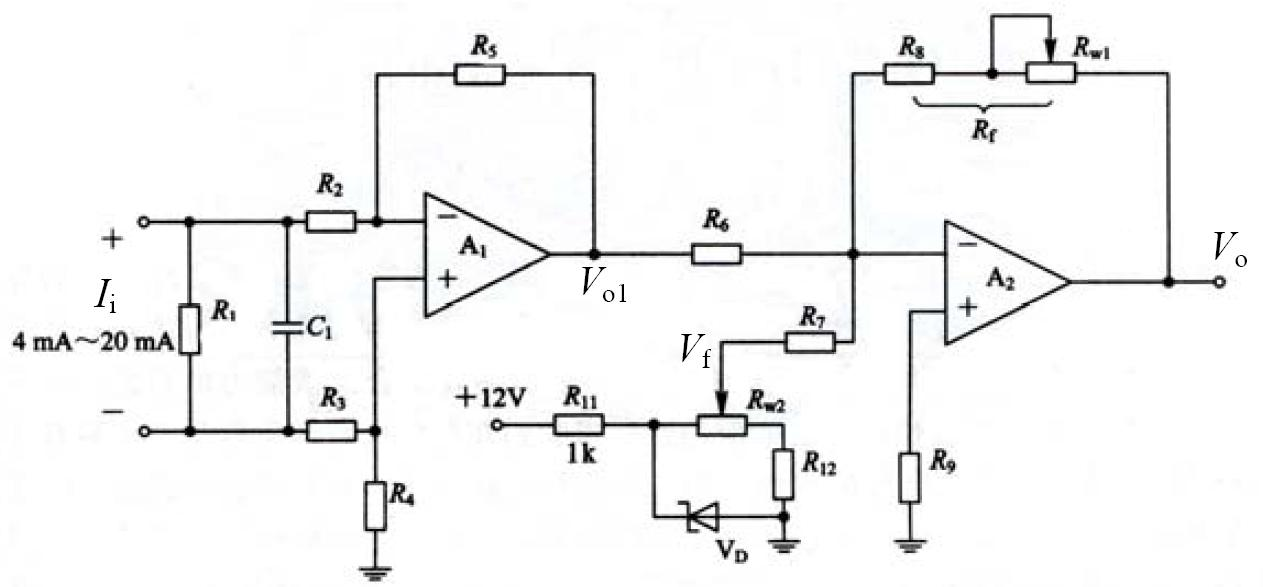
\includegraphics[width=0.96\textwidth]{reference_circuit.png}
  \caption{电流-电压转换参考电路原理图}
  \label{fig:reference-circuit}
\end{figure}

第一级运放 $A_1$ 与 $R_2$、$R_3$、$R_4$、$R_5$ 构成差动放大器。当四个匹配电阻满足
\begin{equation}
  R_2=R_3=R_4=R_5=10\,\mathrm{k}\Omega
  \label{eq:diff-resistors}
\end{equation}
时，差动增益近似为 1。按照图中输入极性约定，第一级输出为
\begin{equation}
  V_{o1} = -I_i R_1 .
  \label{eq:vo1}
\end{equation}
由式 \eqref{eq:vo1} 可得
\begin{equation}
  V_{o1} =
  \begin{cases}
    -1\,\mathrm{V}, & I_i=4\,\mathrm{mA},\\
    -5\,\mathrm{V}, & I_i=20\,\mathrm{mA}.
  \end{cases}
\end{equation}

取样电阻的最大功耗出现在 $I_i=20\,\mathrm{mA}$ 时：
\begin{equation}
  P_{R1,\max}=I_{i,\max}^2R_1
  =(20\times10^{-3})^2\times250
  =0.1\,\mathrm{W}.
  \label{eq:r1-power}
\end{equation}
因此 $R_1$ 宜选用精度较高、额定功率不低于 $1/4\,\mathrm{W}$ 的电阻，以兼顾精度裕量与热稳定性。

\subsection{第二级反相加法与零点平移}

第一级输出 $V_{o1}$ 的范围为 $-1\,\mathrm{V}\sim-5\,\mathrm{V}$，其幅度变化量为 $4\,\mathrm{V}$。目标输出 $V_o$ 的变化量为 $10\,\mathrm{V}$，因此第二级应提供的比例系数为
\begin{equation}
  A_2=\frac{\Delta V_o}{\Delta |V_{o1}|}
  =\frac{10}{4}=2.5 .
  \label{eq:gain-a2}
\end{equation}

第二级 $A_2$ 采用反相加法器结构，对 $V_{o1}$ 和基准电压 $V_f$ 进行加权求和。若反馈电阻为 $R_f$，输入电阻分别为 $R_6$ 和 $R_7$，则
\begin{equation}
  V_o=-\frac{R_f}{R_6}V_{o1}-\frac{R_f}{R_7}V_f .
  \label{eq:adder}
\end{equation}
将式 \eqref{eq:vo1} 代入式 \eqref{eq:adder}，可得
\begin{equation}
  V_o=\frac{R_f}{R_6}I_iR_1-\frac{R_f}{R_7}V_f .
  \label{eq:vo-final}
\end{equation}

为使两个输入支路权重一致，取
\begin{equation}
  R_6=R_7=10\,\mathrm{k}\Omega .
\end{equation}
由式 \eqref{eq:gain-a2} 可知
\begin{equation}
  R_f = 2.5R_6 = 25\,\mathrm{k}\Omega .
  \label{eq:rf}
\end{equation}
实际电路中采用 $R_8=20\,\mathrm{k}\Omega$ 与 $R_{w1}=10\,\mathrm{k}\Omega$ 电位器串联组成可调反馈电阻，便于在调试时补偿元件误差并校准满量程输出。

由 $I_i=4\,\mathrm{mA}$ 时 $V_o=0\,\mathrm{V}$ 的条件，结合 $R_6=R_7$ 与 $R_f/R_6=2.5$，有
\begin{align}
  0 &= 2.5 \times (4\times10^{-3}) \times 250 - 2.5 V_f,\\
  V_f &= 1\,\mathrm{V}.
  \label{eq:vf}
\end{align}
因此理想情况下应将基准调节端 $V_f$ 调至约 $1\,\mathrm{V}$。此时式 \eqref{eq:vo-final} 化为
\begin{equation}
  V_o=2.5\left(I_iR_1 - V_f\right)
  =2.5\left(250 I_i-1\right),
  \label{eq:transfer-designed}
\end{equation}
其与式 \eqref{eq:ideal-transfer} 完全一致。

\subsection{基准电压与补偿电阻计算}

为避免 $V_f$ 直接受电源波动影响，设计中使用 $5.1\,\mathrm{V}$ 稳压二极管产生稳定基准，再经分压与电位器调节得到约 $1\,\mathrm{V}$ 的可调偏置。若稳压电源为 $+12\,\mathrm{V}$，稳压管工作电流取约 $10\,\mathrm{mA}$，分压支路电流取约 $5\,\mathrm{mA}$，则限流电阻估算为
\begin{equation}
  R_{11}\approx
  \frac{12-5.1}{(10+5)\times10^{-3}}
  =460\,\Omega .
  \label{eq:r11}
\end{equation}
原理图中取 $R_{11}=470\,\Omega$，符合常用标称值。分压部分采用 $R_{12}=510\,\Omega$ 与 $R_{w2}=500\,\Omega$，可将 $V_f$ 调节到覆盖 $1\,\mathrm{V}$ 的范围。

反相加法器同相端接地，为减小输入偏置电流引起的输出误差，常在同相端串接补偿电阻 $R_9$。其阻值可按反相端等效电阻估算：
\begin{equation}
  R_9 \approx R_6 \parallel R_7 \parallel R_f .
  \label{eq:r9}
\end{equation}
取 $R_6=R_7=10\,\mathrm{k}\Omega$、$R_f\approx25\,\mathrm{k}\Omega$，有
\begin{equation}
  R_9\approx
  \left(\frac{1}{10\,\mathrm{k}\Omega}
  +\frac{1}{10\,\mathrm{k}\Omega}
  +\frac{1}{25\,\mathrm{k}\Omega}\right)^{-1}
  \approx4.17\,\mathrm{k}\Omega ,
\end{equation}
实际取 $4.3\,\mathrm{k}\Omega$。输入端并联电容 $C_1=100\,\mathrm{pF}$ 用于抑制高频干扰，其与 $R_1$ 构成的近似截止频率为
\begin{equation}
  f_c=\frac{1}{2\pi R_1C_1}
  =\frac{1}{2\pi\times250\times100\times10^{-12}}
  \approx6.37\,\mathrm{MHz}.
\end{equation}
该频率远高于一般工业慢变量信号频段，因此不会影响低频测量响应，主要用于削弱尖峰和高频耦合噪声。

\subsection{理论输出值}

根据式 \eqref{eq:transfer-designed}，典型输入电流对应的理论输出如表 \ref{tab:theoretical-output} 所示。
\begin{table}[H]
  \centering
  \caption{典型输入点的理论转换结果}
  \label{tab:theoretical-output}
  \begin{tabular}{ccccc}
    \toprule
    $I_i/\mathrm{mA}$ & $V_s/\mathrm{V}$ & $V_{o1}/\mathrm{V}$ & $V_f/\mathrm{V}$ & $V_o/\mathrm{V}$ \\
    \midrule
    4  & 1 & -1 & 1 & 0 \\
    8  & 2 & -2 & 1 & 2.5 \\
    12 & 3 & -3 & 1 & 5.0 \\
    16 & 4 & -4 & 1 & 7.5 \\
    20 & 5 & -5 & 1 & 10.0 \\
    \bottomrule
  \end{tabular}
\end{table}

\section{电路与 PCB 设计方案}

\subsection{原理图设计思路}

本设计的实际原理图如图 \ref{fig:schematic} 所示。电路可分为输入取样与差动放大、反相加法与满量程校准、稳压分压与零点校准、供电与测试接口四个模块。

\begin{figure}[H]
  \centering
  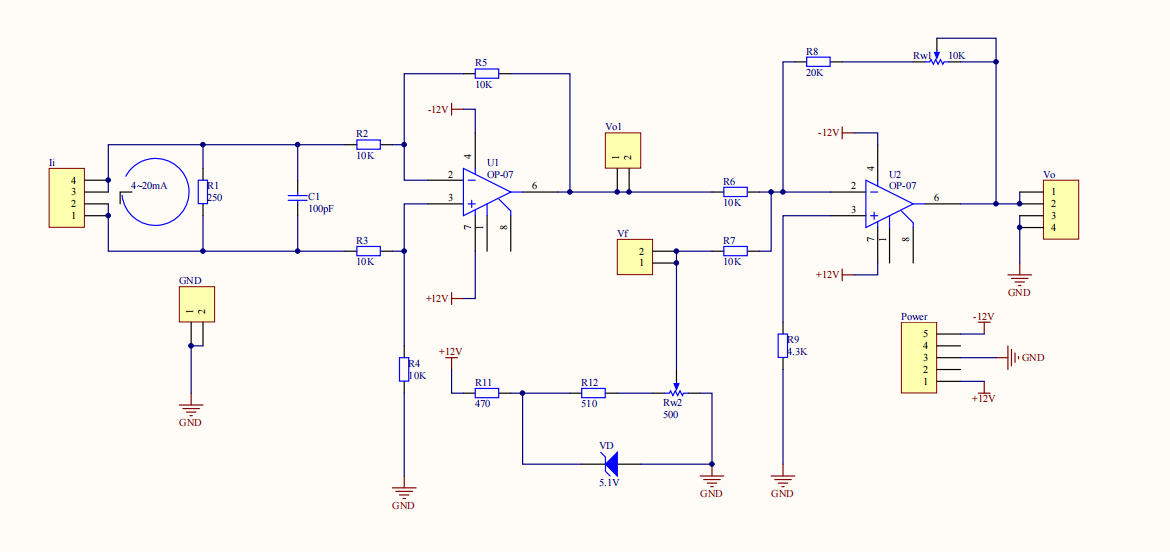
\includegraphics[width=0.98\textwidth]{schematic.png}
  \caption{电流-电压转换电路 Altium 原理图}
  \label{fig:schematic}
\end{figure}

输入端使用四针接口引入 $4\,\mathrm{mA}\sim20\,\mathrm{mA}$ 电流信号。$R_1=250\,\Omega$ 完成电流取样，$C_1=100\,\mathrm{pF}$ 用于高频旁路。第一级运放 U1 采用 OP07，并由 $R_2$、$R_3$、$R_4$、$R_5$ 构成单位增益差动放大结构，将取样电压转换为 $V_{o1}$，同时降低输入端共模扰动对后级的影响。

第二级运放 U2 采用反相加法器结构。$R_6$ 接收第一级输出，$R_7$ 接收基准调节电压 $V_f$，$R_8$ 与 $R_{w1}$ 组成反馈支路。设计时先用理论值确定 $R_f\approx25\,\mathrm{k}\Omega$，再通过电位器在实物调试中完成满量程校准。U2 同相端通过 $R_9$ 接地，减小输入偏置电流在两输入端等效阻抗不一致时造成的输出漂移。

基准电压由 $R_{11}$、稳压二极管 VD、$R_{12}$ 与 $R_{w2}$ 构成。VD 选用 $5.1\,\mathrm{V}$ 稳压管，是因为该电压附近的稳压管温度系数较小，有利于提高零点稳定性。$R_{w2}$ 负责将 $V_f$ 调至约 $1\,\mathrm{V}$，对应 $4\,\mathrm{mA}$ 输入时输出为 $0\,\mathrm{V}$。

\subsection{元器件选型}

主要元器件参数如表 \ref{tab:components} 所示。
\begin{table}[H]
  \centering
  \caption{主要元器件及选型依据}
  \label{tab:components}
  \begin{tabular}{>{\centering\arraybackslash}p{3cm} p{4.3cm} p{6.2cm}}
    \toprule
    元器件 & 取值或型号 & 选型依据 \\
    \midrule
    $R_1$ & $250\,\Omega$ & 标准变送器负载，$4\,\mathrm{mA}\sim20\,\mathrm{mA}$ 对应 $1\,\mathrm{V}\sim5\,\mathrm{V}$ \\
    $R_2,R_3,R_4,R_5$ & $10\,\mathrm{k}\Omega$ & 构成单位增益差动放大器，要求匹配性好 \\
    $R_6,R_7$ & $10\,\mathrm{k}\Omega$ & 反相加法器两个输入支路等权重 \\
    $R_8+R_{w1}$ & $20\,\mathrm{k}\Omega+10\,\mathrm{k}\Omega$ & 形成 $R_f$ 可调范围，便于满量程校准 \\
    $R_9$ & $4.3\,\mathrm{k}\Omega$ & 匹配反相端等效电阻，降低偏置电流误差 \\
    $R_{11}$ & $470\,\Omega$ & 稳压管限流，保证基准支路工作电流 \\
    $R_{12}+R_{w2}$ & $510\,\Omega+500\,\Omega$ & 产生可调 $V_f$，用于零点校准 \\
    $C_1$ & $100\,\mathrm{pF}$ & 抑制输入端高频干扰 \\
    U1、U2 & OP07 & 低失调电压、低漂移，适合精密直流放大 \\
    VD & $5.1\,\mathrm{V}$ 稳压管 & 温度系数较小，适合作基准源 \\
    \bottomrule
  \end{tabular}
\end{table}

\subsection{PCB 布局布线策略}

PCB 设计如图 \ref{fig:pcb-layout} 所示。版图采用左右方向的信号流：输入接口位于左侧，第一级 U1 靠近输入取样网络，第二级 U2 靠近输出端，电源接口布置在右侧，便于供电和测量。这样的布局方式与原理图功能模块一致，可降低连线交叉，提高调试可读性。

\begin{figure}[H]
  \centering
  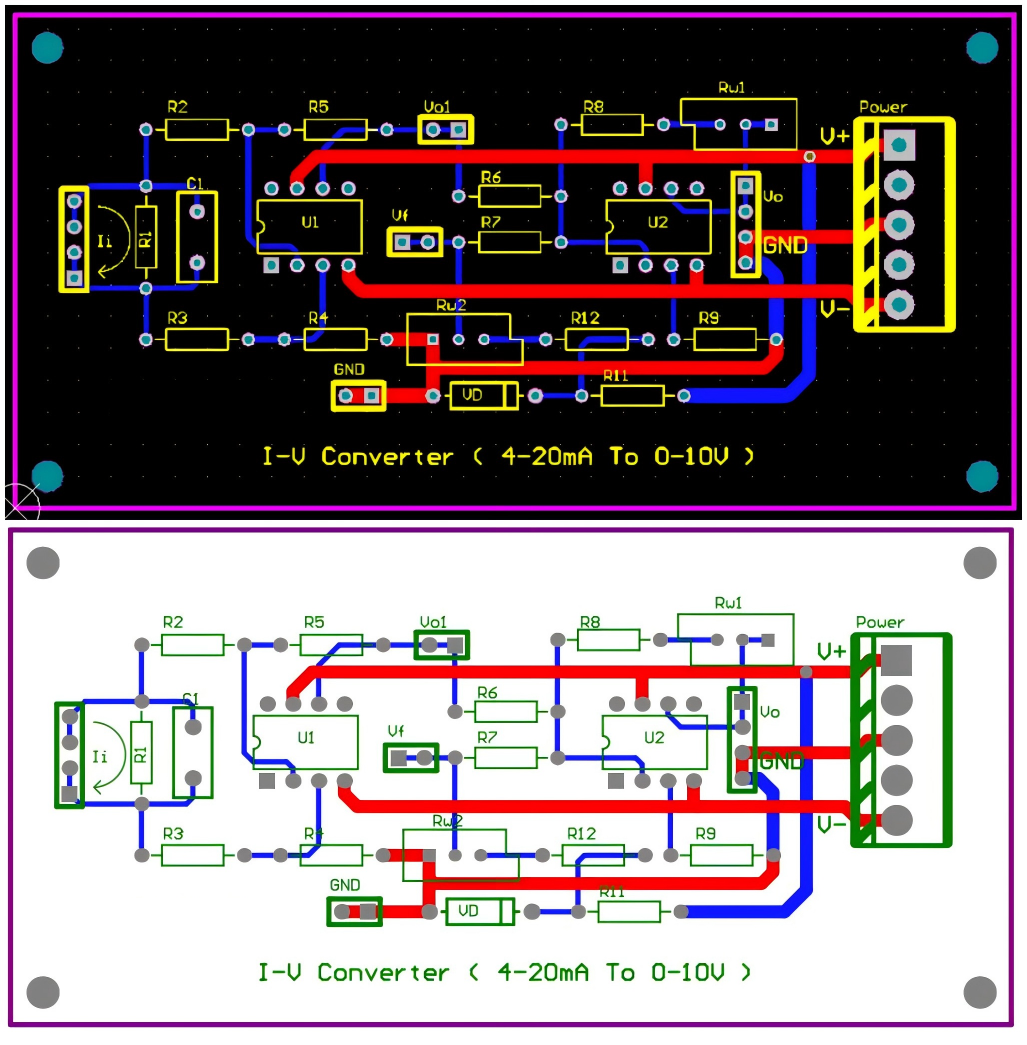
\includegraphics[width=0.82\textwidth]{pcb.png}
  \caption{电流-电压转换电路 PCB 版图与丝印效果}
  \label{fig:pcb-layout}
\end{figure}

布局时应遵循以下原则：
\begin{enumerate}
  \item \textbf{按功能模块集中放置。} 输入取样与 U1 放在左侧，反相加法器与 U2 放在中右侧，稳压分压电路放在下方，减少跨模块长距离绕线。
  \item \textbf{关键测试点外引。} 图中设置了 $V_{o1}$、$V_f$、$V_o$ 和 GND 接口，便于分级调试。若只测最终输出，难以及时判断误差来自第一级、第二级还是基准支路。
  \item \textbf{电源线与地线适当加宽。} PCB 图中电源和地网络采用较宽走线，降低压降与公共阻抗耦合；模拟信号线保持路径短且避免不必要的环路。
  \item \textbf{走线避免直角。} 拐角处使用 $45^\circ$ 过渡，可改善可制造性，也能减少尖角处的工艺缺陷风险。
  \item \textbf{丝印信息完整。} 板上标注了器件编号、电源极性、输入输出端和电路名称，有利于焊接、排错和后续复现。
\end{enumerate}

从图 \ref{fig:pcb-layout} 可见，板边界、安装孔、输入输出接口和电源接口均已预留。由于该电路为低频精密模拟电路，PCB 重点不在高速阻抗控制，而在于地线参考清晰、取样节点短、反馈环路紧凑和调试端口可访问。

\section{实物展示与测试方案}

\subsection{实物展示}

加工后的 PCB 正反面如图 \ref{fig:photos} 所示。正面可见器件丝印、输入端、运放封装位置、反馈电位器和电源接口；背面可见主要铜箔走线和焊盘结构。正反面对照能够检查 PCB 加工是否存在断线、短路、孔位偏移和丝印方向错误等问题。

\begin{figure}[H]
  \centering
  \begin{subfigure}[b]{0.96\textwidth}
    \centering
    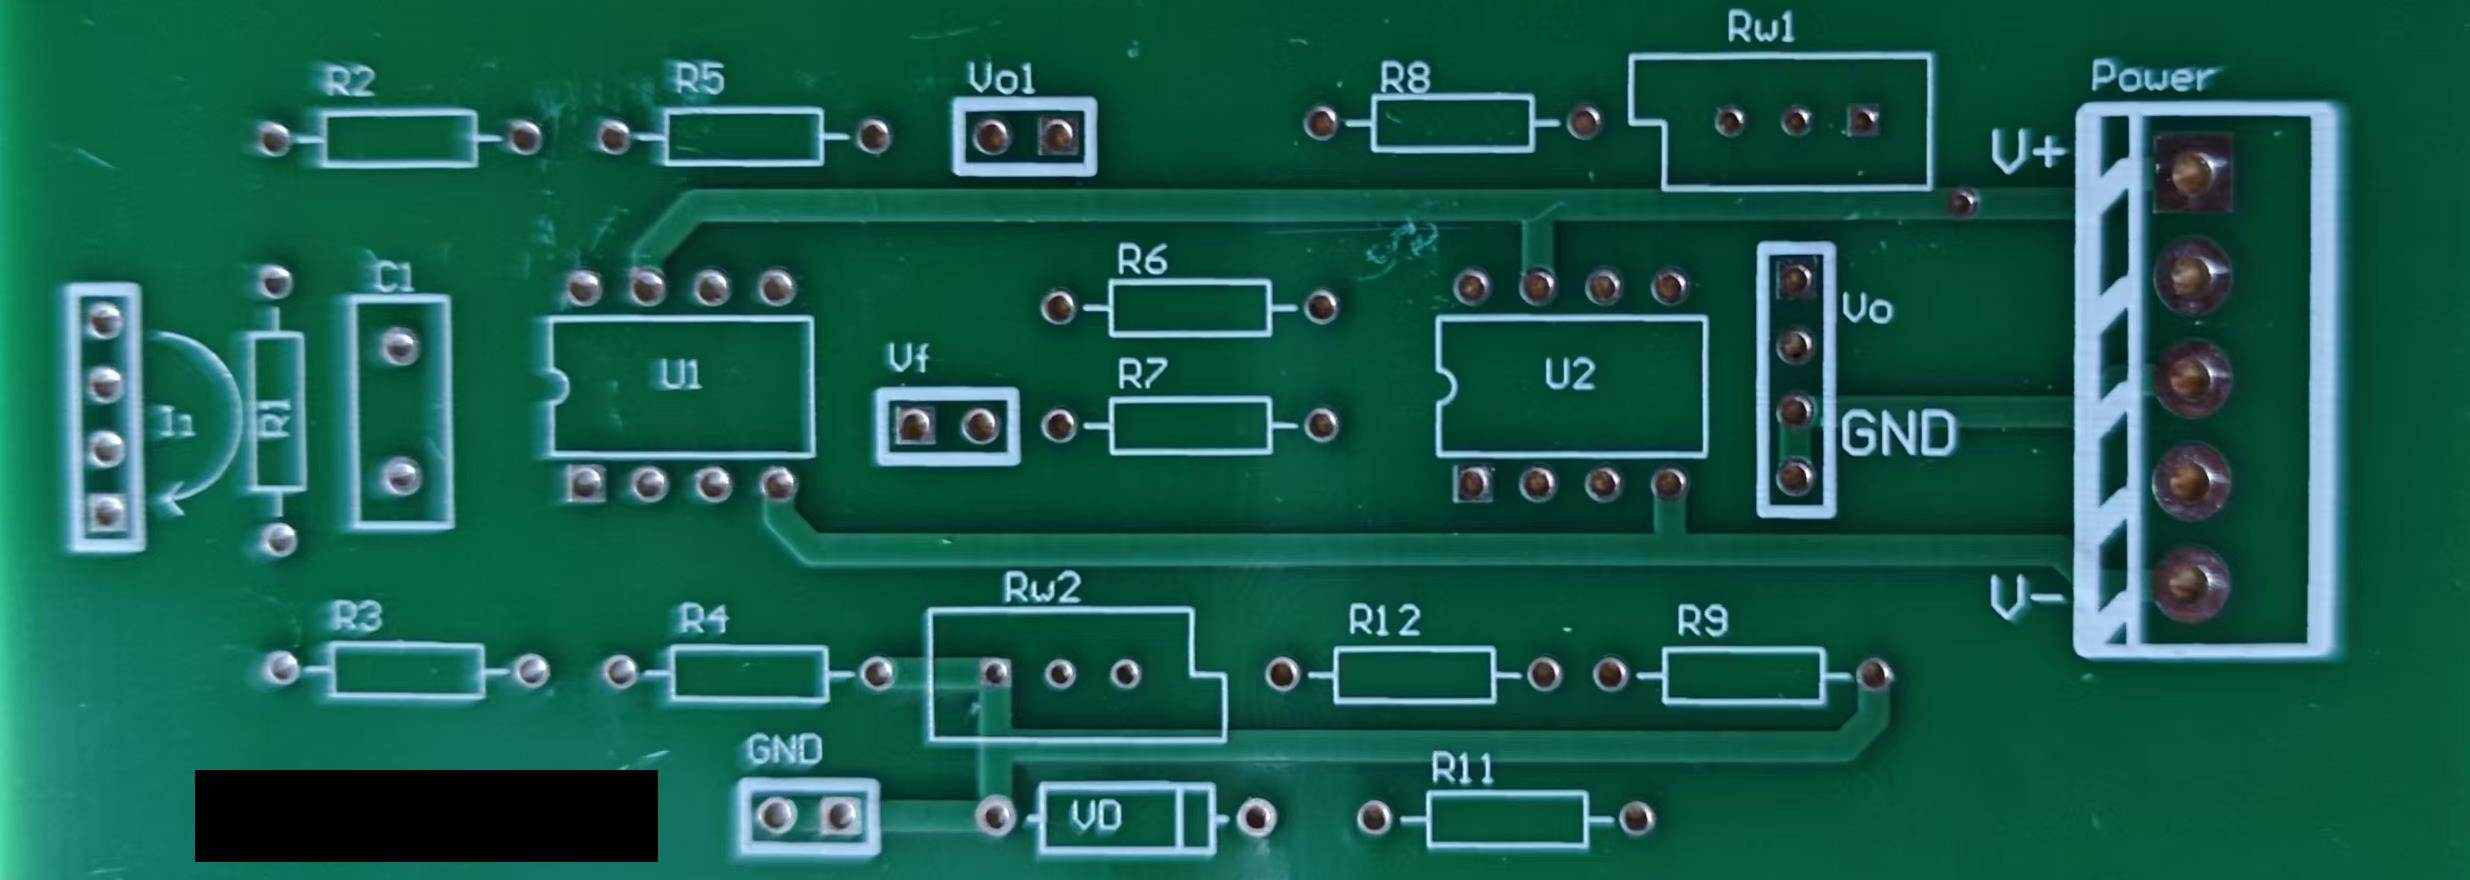
\includegraphics[width=\textwidth]{photo_front_cropped.png}
    \caption{PCB 实物正面}
    \label{fig:photo-front}
  \end{subfigure}
  \vspace{0.4em}
  \begin{subfigure}[b]{0.96\textwidth}
    \centering
    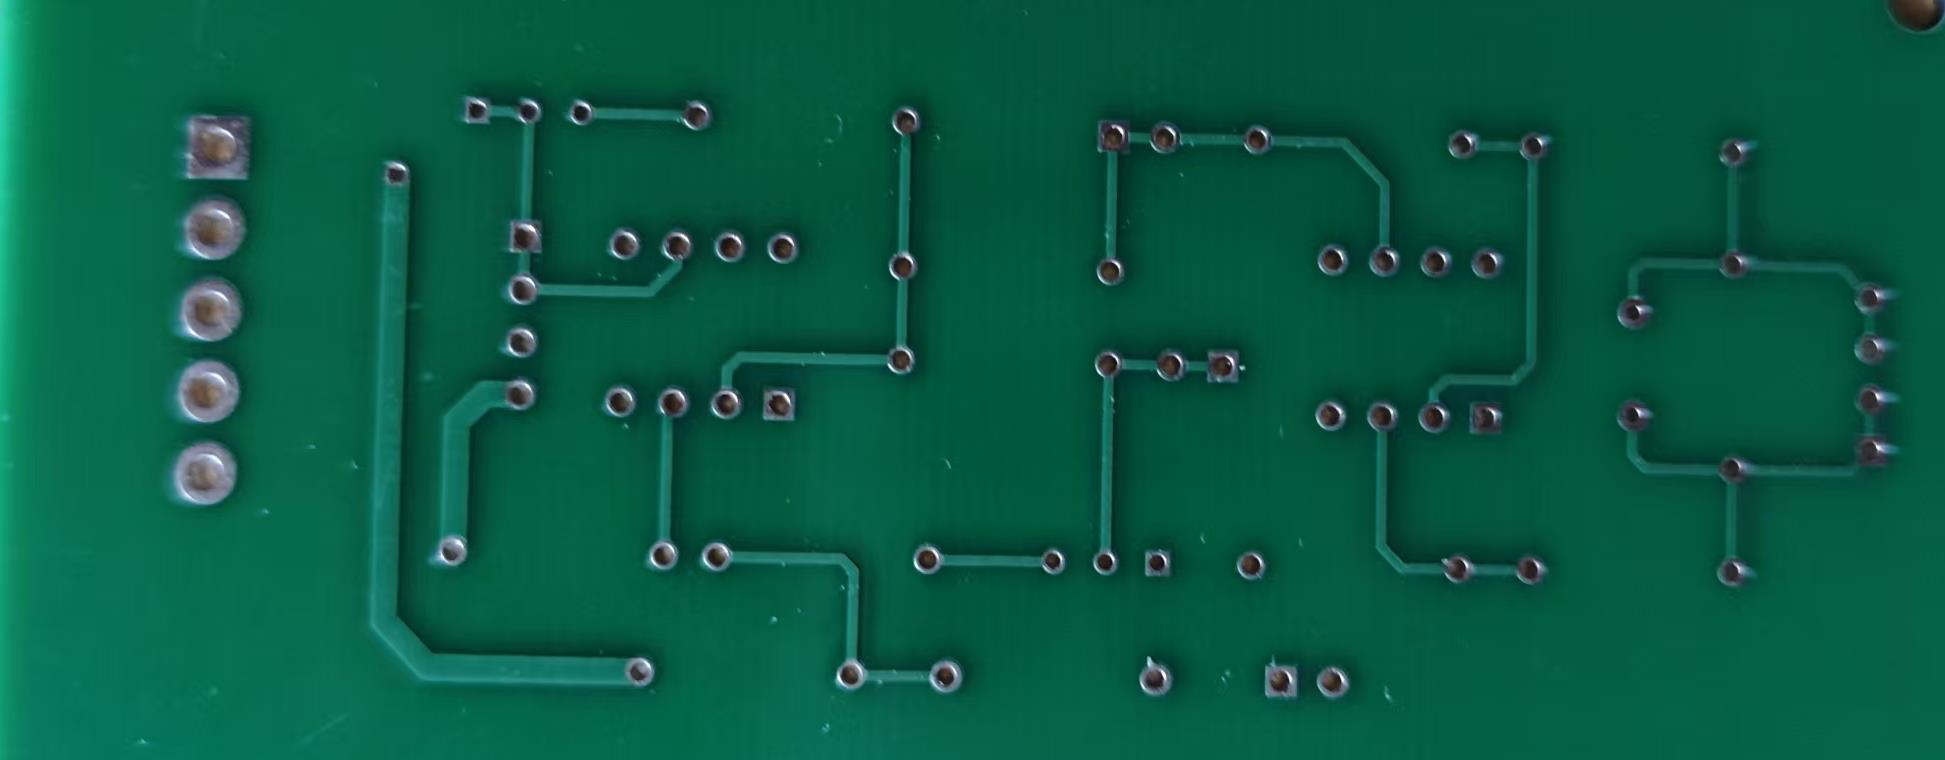
\includegraphics[width=\textwidth]{photo_back_cropped.png}
    \caption{PCB 实物背面}
    \label{fig:photo-back}
  \end{subfigure}
  \caption{电流-电压转换电路实物照片}
  \label{fig:photos}
\end{figure}

\subsection{测试仪器与连接方式}

后续调试建议使用直流稳压电源、可调恒流源或电压源加限流电阻模拟电流源、数字万用表和示波器。测试前应先不插运放芯片，检查 $\pm12\,\mathrm{V}$ 与 GND 是否短路，确认电源接口极性正确后再上电。

调试连接方式如下：
\begin{enumerate}
  \item 将双电源接入 Power 接口，确认 U1、U2 的电源引脚分别得到 $+12\,\mathrm{V}$ 与 $-12\,\mathrm{V}$；
  \item 在输入端接入 $4\,\mathrm{mA}\sim20\,\mathrm{mA}$ 可调电流源；
  \item 用万用表分别测量 $V_{o1}$、$V_f$ 与 $V_o$；
  \item 先调 $R_{w2}$，使 $V_f\approx1\,\mathrm{V}$；再输入 $20\,\mathrm{mA}$，调 $R_{w1}$，使 $V_o\approx10\,\mathrm{V}$；
  \item 回到 $4\,\mathrm{mA}$，检查 $V_o$ 是否接近 $0\,\mathrm{V}$。若偏差较大，重复零点与满量程校准。
\end{enumerate}

\subsection{分级测试方案}

推荐按照“先局部，后整体”的顺序进行测试。第一步仅验证取样与第一级输出，第二步验证基准支路，第三步再联调第二级输出。

\begin{table}[H]
  \centering
  \caption{分级调试与判断依据}
  \label{tab:test-plan}
  \begin{tabular}{>{\centering\arraybackslash}p{2.5cm} p{5.8cm} p{5.5cm}}
    \toprule
    测试阶段 & 测试内容 & 合格判断 \\
    \midrule
    电源检查 & 测量电源接口与运放供电脚 & $+12\,\mathrm{V}$、$-12\,\mathrm{V}$、GND 极性正确，无明显短路 \\
    第一级检查 & 输入 $4\,\mathrm{mA}$ 与 $20\,\mathrm{mA}$，测 $V_{o1}$ & 分别接近 $-1\,\mathrm{V}$ 与 $-5\,\mathrm{V}$ \\
    基准检查 & 调节 $R_{w2}$，测 $V_f$ & 可稳定调至约 $1\,\mathrm{V}$ \\
    满量程校准 & 输入 $20\,\mathrm{mA}$，调节 $R_{w1}$ & $V_o$ 接近 $10\,\mathrm{V}$ \\
    线性检查 & 依次输入 4、8、12、16、20 mA & 输出接近 0、2.5、5、7.5、10 V \\
    \bottomrule
  \end{tabular}
\end{table}

\subsection{误差来源分析}

实际输出误差主要来自以下方面：
\begin{enumerate}
  \item $R_1$ 的阻值误差直接改变取样电压，是转换斜率误差的重要来源；
  \item $R_2$、$R_3$、$R_4$、$R_5$ 匹配不佳会使差动放大器增益偏离 1，并降低共模抑制能力；
  \item $R_f/R_6$ 与 $R_f/R_7$ 的比例误差会同时影响满量程斜率与零点抵消；
  \item OP07 的输入失调电压、输入偏置电流和温漂会在直流精密测量中形成小幅输出漂移；
  \item 稳压管、电位器接触稳定性和电源纹波会影响 $V_f$，从而造成零点偏移；
  \item 焊接质量、接插件接触电阻和测试线连接方式也可能引入附加误差。
\end{enumerate}
因此调试时应优先测量 $V_{o1}$ 与 $V_f$，将误差定位到具体级别，再通过 $R_{w2}$ 和 $R_{w1}$ 分别修正零点和满量程。

\section{设计总结}

本设计围绕 $4\,\mathrm{mA}\sim20\,\mathrm{mA}$ 到 $0\,\mathrm{V}\sim10\,\mathrm{V}$ 的标准信号转换展开。理论上，$250\,\Omega$ 取样电阻先将输入电流转换为 $1\,\mathrm{V}\sim5\,\mathrm{V}$ 的取样电压；第一级差动放大器输出 $-1\,\mathrm{V}\sim-5\,\mathrm{V}$；第二级反相加法器通过 $2.5$ 倍增益和约 $1\,\mathrm{V}$ 基准偏置，实现
\[
  V_o = 625I_i - 2.5 .
\]
原理图设计中通过 OP07、精密电阻、稳压二极管和可调电位器兼顾精度与调试便利性；PCB 设计中按信号流分区布局，保留关键测试点，并通过较宽电源地线与清晰丝印提高可靠性和可维护性。后续实物测试应采用分级校准方法，先验证取样和基准，再校准零点和满量程，最终通过多点测量评估线性度和误差。

\end{document}
